The parameters for the given conic are
\begin{align}
	\label{12/6/3/25eq:V_matrix}
	\vec{V} &= \myvec{0 & 0\\0 & 1},
	\\
	\label{12/6/3/25eq:u_vector}
	\vec{u} &= \myvec{-3/2\\0},
	\\
	\label{12/6/3/25eq:f_value}
	f &= 2
	%\\
\end{align}
which represent a parabola. 
Following the approach in 
\probref{chapters/12/6/3/15},
   \begin{align}
     \vec{p_1} = \myvec{1\\0},\
     \vec{n} = \myvec{-2\\1},
    \end{align}
yielding the matrix equation
\begin{align}
	\label{12/6/3/25eq:vertex_system}
	\myvec{-3&0\\0& 0\\0& 1}\vec{q} = \myvec{-41/16\\0 \\3/4}\\
\end{align}
The augmented matrix for \eqref{12/6/3/25eq:vertex_system} can be expressed as
\begin{align*}
	%\label{12/6/3/25eq:vertex_solv1}
	%\myvec{-3&0&\vrule&2\\0&0&\vrule&0\\0&1&\vrule&0}\\ 	
	%\label{12/6/3/25eq:vertex_solv2}
	\xleftrightarrow[]{R_2 \leftrightarrow R_3}\myvec{-3&0&\vrule&-41/16\\0&1&\vrule&0\\0&0&\vrule&3/4}
	\xleftrightarrow[]{-\frac{R_1}{-3} \leftarrow R_2}\myvec{1&0&\vrule&41/48\\0&1&\vrule&0\\0&0&\vrule&3/4}\\
	\implies\vec{q} = \myvec{\frac{41}{48}\\\frac{3}{4}}
\end{align*}
The equation of tangent is then obtained as
\begin{align}
	\myvec{-2 & 1}\vec{x} +\frac{23}{24} = 0 
\end{align}
See  
		\figref{fig:12/6/3/25}.
	\begin{figure}[!h]
		\centering
 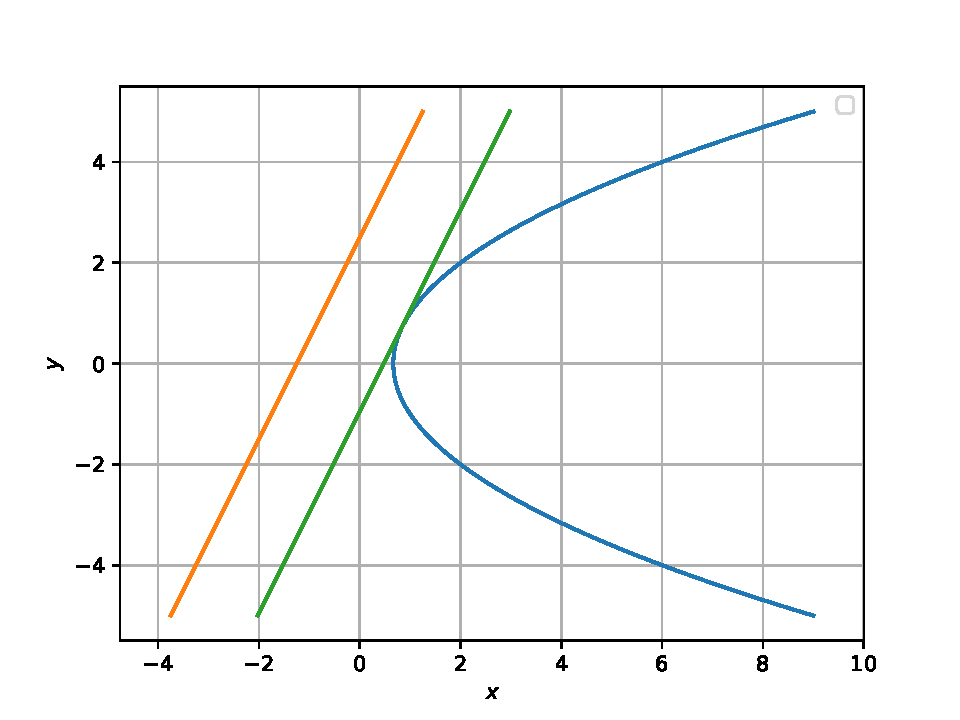
\includegraphics[width=\columnwidth]{chapters/12/6/3/25/figs/conic.pdf}
		\caption{}
		\label{fig:12/6/3/25}
  	\end{figure}
